\documentclass[oneside,a4paper,11pt]{book}

% Packages que usamos
\usepackage[utf8]{inputenc} %idioma
\usepackage[spanish]{babel} %idioma
\usepackage{amsmath} % funciones matemáticas
\usepackage{amssymb} % simbolos matematicos
\usepackage{graphicx} % la portada
\usepackage{fancyhdr} %headers y footers
\usepackage{cite} %bibliografía
\usepackage{emptypage} %modificar páginas
\usepackage{afterpage} %modificar páginas
\usepackage{algorithm} %incluir pseudocodigo
\usepackage{algpseudocode} %incluir pseudocodigo
\usepackage{float}  % para que los algorithm se coloquen bien
\usepackage[colorlinks=false,pdfborder={0 0 0},hidelinks]{hyperref} % Las referencias te llevan a ellas
\usepackage{multirow} % Para las tablas que fusionan celdas
\usepackage{eurosym} % Simbolo del euro

\decimalpoint % usar . en lugar de , para decimales
	
% Re-usable information
\newcommand{\myTitle}{Estudio e implementación paralela de métodos explícitos multipaso}
\newcommand{\mySubTitle}{Resolución de Ecuaciones de Advección-Reacción-Difusión}
\newcommand{\myDegree}{Grado en Ingeniería Informática}
\newcommand{\myName}{José Manuel Navarro Cuartero}
\newcommand{\myProf}{José Miguel Mantas Ruiz}
\newcommand{\myFaculty}{Escuela Técnica Superior de Ingenierías Informática y de Telecomunicación}
\newcommand{\myFacultyShort}{E.T.S. de Ingenierías Informática y de Telecomunicación}
\newcommand{\myDepartment}{Departamento de Lenguajes y Sistemas Informáticos}
\newcommand{\myUni}{Universidad de Granada}

\addto\captionsspanish{ % Renombrar una serie de conceptos
	\renewcommand{\tablename}{Tabla}
	\renewcommand{\contentsname}{Índice}
	\renewcommand{\listtablename}{Listado de Tablas}
	\renewcommand{\listfigurename}{Listado de Figuras}
	\renewcommand{\listalgorithmname}{Listado de Algoritmos}
}

\floatname{algorithm}{Algoritmo} % Renombra los algorithm

\begin{document}
	
	% ============================================
	% 1. PORTADA, PREFACIO E ÍNDICE
	% ============================================
	
	\pagestyle{empty}      % Oculta el número
	\setcounter{page}{1}   % Empieza a contar desde la portada
	
	\input{prefacios/portada}
	\chapter*{}
%\thispagestyle{empty}
%\cleardoublepage

%\thispagestyle{empty}

%\input{portada/portada_2}



%\cleardoublepage
\thispagestyle{empty}

\begin{center}
{ \large\bfseries \myTitle : \\ \mySubTitle } \\
\end{center}
\begin{center}
\myName \\
\end{center}

%\vspace{0.7cm}
\noindent{\textbf{Palabras clave}: palabra\_clave1, palabra\_clave2, palabra\_clave3, ......}\\

\vspace{0.7cm}
\noindent{\textbf{Resumen}}\\

Poner aquí el resumen.
\cleardoublepage


\thispagestyle{empty}


\begin{center}
{\large\bfseries Project Title: Project Subtitle}\\
\end{center}
\begin{center}
First name, Family name (student)\\
\end{center}

%\vspace{0.7cm}
\noindent{\textbf{Keywords}: Keyword1, Keyword2, Keyword3, ....}\\

\vspace{0.7cm}
\noindent{\textbf{Abstract}}\\

Write here the abstract in English.

\chapter*{}
\thispagestyle{empty}

%\noindent\rule[-1ex]{\textwidth}{2pt}\\[4.5ex]

Yo, \textbf{ \myName }, alumno de la titulación \textbf{\myDegree} de la \textbf{ {\myFaculty} de la {\myUni} }, con DNI 75896777C, autorizo la
ubicación de la siguiente copia de mi Trabajo Fin de Grado en la biblioteca del centro para que pueda ser
consultada por las personas que lo deseen.

\vspace{6cm}

\noindent Fdo: {\myName}

\vspace{2cm}

\begin{flushright}
Granada a X de Septiembre de 2026.
\end{flushright}


\chapter*{}
\thispagestyle{empty}

%\noindent\rule[-1ex]{\textwidth}{2pt}\\[4.5ex]

D. \textbf{\myProf}, Profesor del Área de XXXX del {\myDepartment} de la {\myUni}.

\vspace{0.5cm}

\textbf{Informa:}

\vspace{0.5cm}

Que el presente trabajo, titulado\textbf{ \myTitle , \mySubTitle },
ha sido realizado bajo su supervisión por \textbf{\myName}, y autorizo la defensa de dicho trabajo ante el tribunal
que corresponda.

\vspace{0.5cm}

Y para que conste, expide y firma el presente informe en Granada a X de Septiembre de 2026.

\vspace{1cm}

\textbf{El director:}

\vspace{5cm}

\noindent \textbf{ \myProf }

\chapter*{Agradecimientos}
\thispagestyle{empty}
\vspace{1cm}


Poner aquí agradecimientos...


	
	% Índice 
	\tableofcontents
	
	% ============================================
	% 2. CAPÍTULOS 
	% ============================================
	
	\pagestyle{fancy}
	\fancyhf{}
	\renewcommand{\headrulewidth}{0pt}
	\fancyfoot[C]{\thepage} % Numero en el centro del pie de pagina
	
	\creaCapitulo{Introducción}

Los métodos numéricos son un conjunto de técnicas y algoritmos matemáticos diseñados para encontrar soluciones aproximadas a problemas que, en muchos casos, no pueden resolverse de manera exacta mediante el análisis o su resolución sería muy costosa. Se utilizan asiduamente en diversos campos de la ciencia, ingeniería, economía y muchas otras disciplinas para resolver ecuaciones diferenciales, integrales, sistemas de ecuaciones, aproximación e interpolación, integración numérica entre otros. Es en el primero de estos casos en el que nos centraremos. Si bien es cierto que existen diversas técnicas para la resolución de ecuaciones diferenciales ordinarias y de sistemas de ecuaciones diferenciales, éstas solo se pueden aplicar cuando dichas ecuaciones se ajustan a un patrón concreto.

En el mundo de los métodos numéricos hay infinidad de formas de resolver las EDOs, y tantas o más aplicaciones de las mismas a problemas del mundo real. Escoger el método correcto tiene que ver tanto con la exactitud de la solución, como con su coste, de potencia de computación y tiempo. 

Es en este último punto en el que nos centraremos en los siguientes capítulos, ya que si bien para problemas pequeños, algo tan simple como el método de Euler explícito podría bastarnos, posteriormente plantearemos problemas mucho más complejos, que requerirán soluciones que estén a la altura. Por tanto, no se trata solamente de hallar una solución, sino de hacerlo rápida y eficientemente.

Para esto, partiremos de 4 problemas cuya implementación secuencial y soluciones esperadas ya conocemos de forma previa, y aplicaremos para su resolución 3 métodos numéricos distintos, que a su vez implementaremos con dos tecnologías para paralelizar distintas, OpenMP y CUDA, es decir, paralelismo a nivel de CPU y GPU.

Nuestro objetivo será implementar de forma fiel y exacta tanto los problemas como los métodos de resolución, para posteriormente poder comparar las ganancias en tiempo de ejecución al pasar de una tecnología a otra.

La idea detrás de todo esto es relativamente simple; un algoritmo que utilice 4 o 16 hebras será mejor que uno secuencial. Y uno que utilice 256 será mejor que todos ellos. Aunque la realidad no siempre va de la mano de nuestras ideas, buscaremos conseguir las mayores ganancias aprovechando al máximo todas las herramientas que ponen a nuestra disposición tanto CUDA como OpenMP. Haremos por tanto una serie de mediciones y buscaremos probar nuestra hipótesis.



 % Capitulo 1
	\chapter{Conceptos previos}

\section{Métodos Numéricos y Ecuaciones Diferenciales Ordinarias}

Una ecuación diferencial es aquella que relaciona una función ( $f(x)$ ó $y$), sus variables ($x$) y sus derivadas ( $f’(x)$, $dy/dx$ ó $y’$ ). Para resolver una ecuación diferencial se debe encontrar una función que satisfaga dicha ecuación.
Dentro de las ecuaciones diferenciales nos encontramos las ecuaciones diferenciales ordinarias, EDOs, que contienen derivadas respecto a una sola variable independiente. Más adelante nos centraremos en este tipo en particular. En oposición a éstas estarían las ecuaciones en derivadas parciales, en las que la función $f(x)$ depende de más variables independientes. \cite{Molero2007}

El orden de una ecuación diferencial equivale al orden de la mayor derivada que aparece en la ecuación. Además, será lineal cuando la variable dependiente y todas sus derivadas son de primer grado (no puede haber $f(x)^2$ ), y los coeficientes de la variable dependiente y sus derivadas dependen de la variable independiente.

A modo de ejemplo simple podríamos considerar una ecuación diferencial ordinaria de primer orden como:

\begin{equation}
	\frac{dy}{dt} = -2y \text{ , } y(0)=1
\end{equation}

Donde además de la EDO, se nos está dando su valor inicial. En este caso en particular, sabemos de forma analítica que su solución exacta es $y(t) = e^{-2t}$, y podríamos por tanto calcular cualquier $y(t_n)=y_n$ que deseemos. No obstante, si por cualquier razón no pudiéramos resolverla analíticamente deberíamos recurrir a los métodos numéricos. A través de ellos, y partiendo del valor $y_n$ que se nos proporciona, calcularíamos de forma iterativa $y(t_{n+h})$ hasta llegar al valor $t_n=t_f$ que busquemos como estado final. 

\textbf(DIBUJAR FIGURA AVANCE PASO A PASO)

Podríamos utilizar para EDOs con valor inicial, por ejemplo, el método de Euler, del que hablaremos más adelante. Antes de ello podemos entrar en algo más de detalle respecto a algunos otros conceptos que iremos usando. 


\section{Tipos de métodos numéricos}

Podemos dividir a los métodos en tres grupos, explícitos, implícitos y semiimplícitos. La división se hará en función de cómo se consigue el siguiente paso, es decir, de cómo obtenemos $y_{n+1}$ a partir de $y_n$; de si aparecen valores futuros o no en la fórmula que lo calcula. Tendremos como expresión general la siguiente: \cite{Molero2007}

\begin{equation}
	\label{eq:ExpresionGeneralMetodosUnPaso}
	y_{n+1} = y_n + \Delta t \cdot \Phi (x_n, y_n, y_{n+1}, \Delta t)
\end{equation}

En la cual será la función incremento $\Phi$ la que dirima a cuál de los grupos pertenece el método con el que estemos trabajando.

Los métodos explícitos son aquellos en los que siguiente término se puede obtener directamente, sólo haciendo cálculos con datos de los que ya se dispone. Dicho de otra forma, son aquellos en los que $y_{n+1}$ no aparece en $\Phi$, sólo aparece en la parte izquierda de la ecuación. Entre ellos nos encontraremos el Euler explícito, Runge-Kutta, o Adams-Bashforth, los tres los veremos posteriormente. Los métodos explícitos suelen ser más fáciles de implementar, ya que no requieren resolver ecuaciones, y suelen ser más rápidos. Por otro lado, tienden a ser menos estables, especialmente en problemas rígidos (\textit{stiff}).

Al otro lado del espectro nos encontraríamos a los métodos implícitos, que son aquellos en los que $y_{n+1}$ sí aparece en la parte de la derecha de la igualdad, lo cuál nos obligaría a resolver una ecuación que podrá ser, o no, lineal. Estos métodos son muy estables, y son más adecuados para resolver problemas rígidos (\textit{stiff}). Como parte negativa tienen que requieren resolver ecuaciones en cada paso, y a veces de forma iterativa, lo que los acaba haciendo mucho más costosos computacionalmente. Entre ellos nos encontramos algunos métodos como el Euler implícito, Adams-Moulton, o los métodos BDF. 

Como tercer grupo tendríamos los métodos semiimplícitos. Éstos representan una especie de "solución" a los diferentes problemas que traen consigo los métodos explícitos e implícitos. En este grupo, aunque existe una parte implícita, ésta es más simple, ya que o bien la ecuación a resolver es lineal, o bien se separa la parte rígida para tratarla implícitamente y el resto se trata de forma explícita. Esto es útil cuando el problema tiene términos rígidos (\textit{stiff}) como la difusión, que deben tratarse implícitamente para que el método sea estable incluso con pasos de tiempo grandes, y términos suaves o de comportamiento hiperbólico como la advección, que se pueden tratar explícitamente para evitar resolver sistemas grandes o no lineales.
Los métodos semiimplícitos representan un compromiso entre la estabilidad de los explícitos y la velocidad de los implícitos. Como hemos mencionado, podremos dividir a la EDO en dos partes:

\begin{equation}
	\label{eq:EcuacionSemiimplicita}
	y' = f(x,y) = f_E(x,y) + f_I(x,y)
\end{equation}

En este ejemplo $f_E$ es la parte explícita, suave (no \textit{stiff}), y $f_I$ es la parte que queremos tratar implícitamente. Algunos métodos semiimplícitos son los métodos IMEX (\textit{implicit-explicit})\cite{Ascher1995}, los métodos linealmente implícitos Runge-Kutta (\textit{LIRK})\cite{Calvo2001}, o el método Adams-Bashforth-Moulton (AB-AM predictor-corrector). Es con este último con el que trabajaremos. 

Otra categorización con la que trabajaremos serán los métodos de un solo paso, y los métodos multipaso.
En los métodos de un solo paso, para obtener el siguiente valor con el que se tratará, el siguiente paso, sólo se utiliza información relativa al paso anterior. Es decir, como podemos ver en \ref{eq:ExpresionGeneralMetodosUnPaso}, para obtener $y_{n+1}$ sólo se utilizaría $y_n$.

Sin embargo, los métodos multipaso usan varios valores anteriores de la solución para calcular el siguiente paso en el tiempo, en lugar de basarse solo en el valor actual. Es decir, que para obtener $y_{n+1}$ se podrían tomar pasos intermedios que posteriormente se desechen (como en Runge-Kutta), o utilizar pasos más antiguos como $y_{n-1}$ o $y_{n-2}$. Para problemas de gran tamaño, los métodos multipaso permiten alcanzar resultados con gran precisión y de una forma más eficiente que los métodos de un paso como el de Euler o el de Runge-Kutta.


\section{Método de Euler}

Como hemos comentado, el método de Euler es uno de los métodos numéricos más simples de los que disponemos para la resolución de EDOs. Se trata de un método explícito de un solo paso que se construye a partir de una sencilla idea geométrica: aproximar el valor de la solución en cada nodo por el valor que proporciona la recta tangente a la solución trazada desde el punto correspondiente al nodo anterior.\cite{Gallardo2018} 

\begin{figure}[H]
	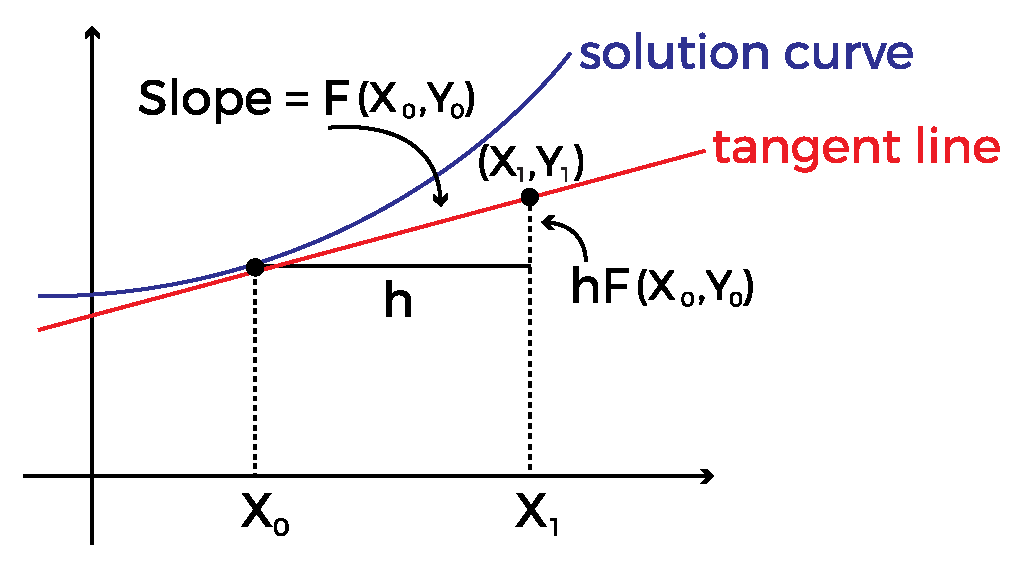
\includegraphics[width=\linewidth]{imagenes/Ejemplo-Euler.png}
	\caption{Aplicación del método de Euler \cite{Calcs2023}}
	\label{fig:Ejemplo-Euler}
\end{figure}

Emplearíamos la siguiente fórmula, aunque puede aparecer escrita de distintas formas equivalentes, aquí mostramos dos:

\begin{equation}
	\label{eq:EulerExplicito}
	\begin{split}
		y_{n+1} &= y_n + \Delta t \cdot f(t_n,y_n) \\
		y_{n+1} &= y_n + h \cdot f(x_n,y_n)
	\end{split}
\end{equation}

Aplicando la misma al ejemplo de valor inicial que mencionamos antes, $\frac{dy}{dt} = -2y \text{ , } y(0)=1$, sabemos que $y_n$ corresponde a la aproximación numérica de $y(t_n)$, y $\Delta t$ (o $h$) representa la variación en el tiempo paso a paso que estemos considerando. Además, en nuestro caso, $f(t_n,y_n)$ sería $-2 \cdot y_n$, y se nos da el valor inicial $t_0 = 0.0$. Por tanto, tomando estos valores, con un $\Delta t = 0.1$, y $t_f = 1.0$, calcularemos los sucesivos valores para $t = 0.1, 0.2, ..., 1.0$.

El primer paso sería por tanto, partiendo de los valores iniciales, calcular el $t=0.1$, a saber, $y_1 = y_0 + \Delta t \cdot f(t_0,y_0) = 1 + 0.1 \cdot (-2 \cdot 1) = 0.8 $. Si esto lo repitiéramos de forma sucesiva obtendríamos los siguientes resultados, los cuales además compararemos con el valor real $y(t) = e^{-2t}$ para obtener el error absoluto $\varepsilon_a$ y el error relativo $\varepsilon_r$. Definiremos al error absoluto como la diferencia entre el valor real y nuestra aproximación, y al error relativo como el cociente entre el error absoluto y el valor real, en porcentaje.

\begin{table}[H]
	\begin{center}
		\begin{tabular}{| c | c | c | c | c | c |}
			\hline
			Paso $n$ & $t_n$ & $y_n$(Euler) & $y_n$(Exacta) & $\varepsilon_a$ & $\varepsilon_r$ \\ \hline
			0  & 0.0 & \multicolumn{2}{c|}{Valor Inicial = 1.0} & - & - \\
			1  & 0.1 & 0.8     & 0.81873 & 0.01873 &  2.29 \\
			2  & 0.2 & 0.64    & 0.67032 & 0.03032 &  4.52 \\
			3  & 0.3 & 0.512   & 0.54881 & 0.03681 &  6.71 \\
			4  & 0.4 & 0.4096  & 0.44933 & 0.03973 &  8.84 \\
			5  & 0.5 & 0.32768 & 0.36788 & 0.04020 & 10.93 \\
			6  & 0.6 & 0.26214 & 0.30119 & 0.03905 & 12.97 \\
			7  & 0.7 & 0.20972 & 0.24660 & 0.03688 & 14.96 \\
			8  & 0.8 & 0.16777 & 0.20190 & 0.03412 & 16.90 \\
			9  & 0.9 & 0.13422 & 0.16530 & 0.03108 & 18.80 \\
			10 & 1.0 & 0.10737 & 0.13534 & 0.02796 & 20.66 \\ \hline
		\end{tabular}
		\caption{Comparativa entre Euler y valor real}
		\label{tab:Comparativa-Euler}
	\end{center}
\end{table}

\begin{figure}[H]
	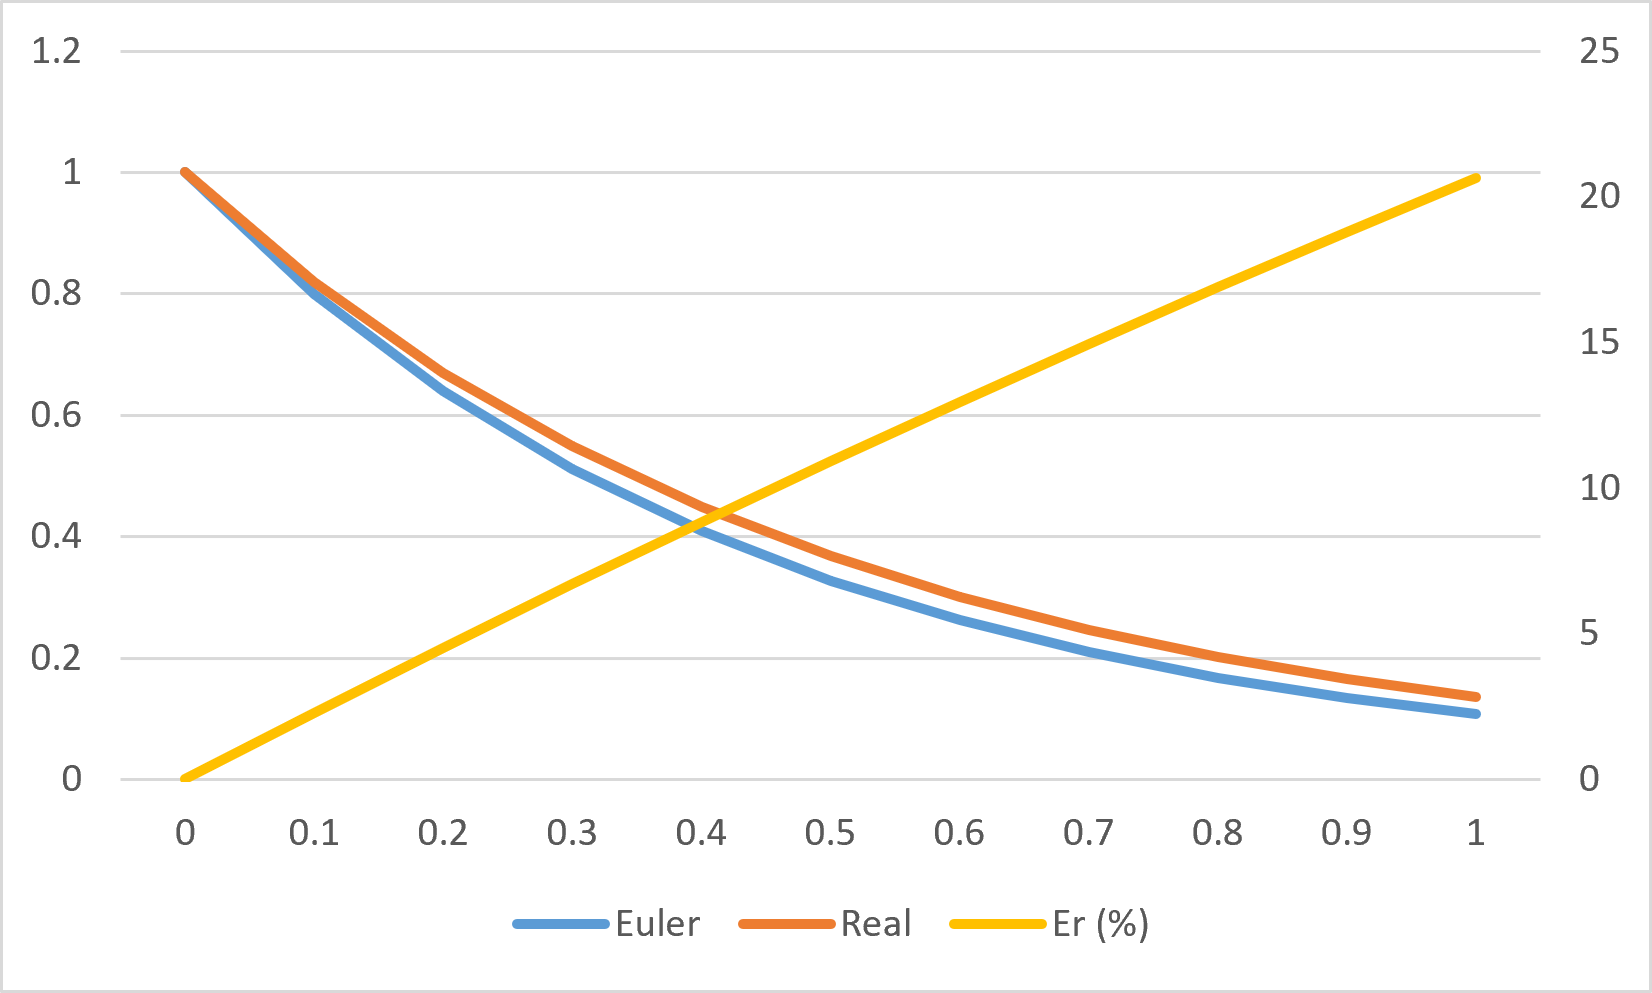
\includegraphics[width=\linewidth]{imagenes/Comparativa-Euler.png}
	\caption{Comparativa entre Euler y valor real}
	\label{fig:Comparativa-Euler}
\end{figure}

Como podemos observar en la tabla \ref{tab:Comparativa-Euler} y en la figura \ref{fig:Comparativa-Euler}, los valores que obtenemos con el Euler explícito son próximos a los reales (eje Y izquierdo); el error absoluto se mantiene estable por debajo de 0.05, e incluso disminuye. Sin embargo, el error relativo (eje Y derecho) aumenta de forma lineal con cada iteración, y para la última alcanza un preocupante 20\%. Esto nos indica que para este problema, quizás el método numérico que hemos utilizado o el $\Delta t$ que hemos considerado no son los más indicados. 

\section{Paralelismo}
Las dos tecnologías que vamos a utilizar para introducir el paralelismo en nuestro código y las mejoras que trae consigo son OpenMP y CUDA, es decir, paralelismo a  nivel de CPU, y a nivel de GPU, respectivamente.

Por muy rápida que sea nuestra CPU, siempre llegaremos a un punto en que, bien por la complejidad de los problemas, bien por el tamaño que se maneje, una sola CPU con un código secuencial no va a ser suficiente. Es aquí donde entra el paralelismo, y es aquí donde nos centraremos.

La programación paralela es el conjunto de técnicas, modelos y arquitecturas que permiten ejecutar múltiples operaciones de forma simultánea, explotando el hardware moderno (CPU multicore, GPU masivamente paralelas, aceleradores, clústeres). Su objetivo es reducir el tiempo de ejecución, aumentar el rendimiento y permitir resolver problemas que, como hemos comentado, serían inviables en código secuencial.

El paralelismo surge cuando un problema puede descomponerse en subtareas independientes que pueden ejecutarse al mismo tiempo. En términos formales, un programa es paralelizable si existe una partición de su espacio de trabajo en unidades que no presentan dependencias de datos que impidan su ejecución concurrente. Esto implica analizar dependencias de datos, localidad y acceso a memoria, granularidad de las tareas, y coste de sincronización.

Podríamos clasificar los distintos modelos de paralelismo que nos encontraremos de la siguiente forma. Por un lado tendríamos el paralelismo de datos, que consiste en aplicar la misma operación a múltiples elementos de un conjunto, a través de la vectorización, de bucles paralelos, o de operaciones \textit{element-wise}. Dentro de esta categoría nos encontraríamos a OpenMP, CUDA, OpenCL, o AVX, entre otros.

Por otro lado tendríamos el paralelismo de tareas, que consiste en ejecutar tareas heterogéneas en paralelo, como pipelines, árboles de tareas, o grafos de dependencias. Este modelo es usado por frameworks como TBB, Cilk, OpenMP tasks o runtimes de grafos. Por último el paralelismo híbrido combina ambos, buscando el paralelismo de tareas, con paralelismo de datos dentro de cada tarea.

Algunos conceptos muy importantes que nos encontraremos son la concurrencia y el paralelismo. La concurrencia hace referencia a que varias tareas pueden ocurrir a la vez, o que ocurren simultáneamente de forma lógica. Una CPU \textit{single-core} puede cambiar rápidamente de una tarea a otra si no tienen dependencia entre ellas y son concurrentes. Mientras que el paralelismo trata sobre ejecutar físicamente varias tareas al mismo tiempo, por ejemplo a través de varios núcleos (como en OpenMP) o de varias hebras (como en CUDA).

El speedup será la forma en la que mediremos las mejoras en la ejecución conforme aumenta el paralelismo. En nuestro caso, lo calcularemos dividiendo el tiempo de ejecución del programa secuencial, entre el paralelizado.\cite{Schryen2024} Como todo código por bien optimizado que esté va a tener una parte secuencial que no pueda paralelizarse, buscaremos que el speedup aumente tanto como sea posible. Por ejemplo, pasando de un código secuencial a uno con 4 hebras OpenMP, el speedup ideal sería de 4, aunque entendemos que no será posible conseguirlo, pero sí acercarse lo suficiente. 

Otro concepto relacionado sería el de la eficiencia, que sería el cociente entre speedup y el número de cores, o de hebras, empleado para obtener ese speedup. La eficiencia estará entre 0 y 1 (o entre 0\% y 100\%), y medirá cuánto se están aprovechando los recursos paralelos.

Al hilo de esto último, la Ley de Amdahl \cite{Amdahl1967} nos indica que, con un tamaño de problema constante y aumentando el número de procesadores, la parte no paralelizable del programa va a limitar nuestro speedup. Podemos ilustrarla tal que:

\begin{equation}
	\label{eq:LeyAmdahl}
	S(p) = \frac{1}{ (1-f) + f/p }
\end{equation}

Siendo $p$ el numero de procesadores, $f$ la fracción paralelizable del programa, $1-f$ por tanto sería la parte secuencial, y $S(p)$ sería el speedup máximo teórico. La interpretación que podemos hacer es que cuando aumentan los hilos, la parte no paralelizable satura el speedup. Por ejemplo, con un 95\% del programa paralelizable, e infinitos procesadores, el speedup nunca superará 20. Trayendo esto a un contexto más realista, lo que se nos indica es que, aunque obviamente aumentar los núcleos o los hilos es efectivo, y reduciremos los tiempos de ejecución, llegará un número a partir del cual ya no merezca la pena.

También debemos mencionar la Ley de Gustafson \cite{Gustafson1988}, que parte de una premisa distinta, aumentar el tamaño del problema cuando tenemos más procesadores. A saber:

\begin{equation}
	\label{eq:LeyGustafson}
	S(p) = p - (1-f) \cdot (p-1)
\end{equation}

Aquí la interpretación que hacemos es que al aumentar el tamaño del problema, aumentamos la parte paralelizable, mientras que la secuencial se mantiene estable. Esto juega a nuestro favor, ya que trataremos grandes cantidades de datos. La ley de Gustafson aporta un punto de vista más optimista al binomio procesadores-eficiencia, ya que nos dice que aunque la eficiencia no pueda ser perfecta, a medida que el problema y los hilos crezcan, podrá acercarse mucho.

Otro concepto importante será el de la sincronización. Cuando hilos diferentes deban compartir algún dato entre ellos, o necesiten que haya terminado cierta tarea antes de empezar la siguiente, deberá haber una barrera en la que los hilos se esperen entre ellos. Estas barreras ralentizan mucho la ejecución y se deberá intentar reducirlas tanto como sea posible. % Capitulo 2.1 a 2.4
	\creaCapitulo{Métodos de Resolución}
Para resolver los diferentes problemas hemos implementado tres métodos distintos, a saber: Runge-Kutta, que es explícito y utiliza pasos intermedios ($K1, K2$) para obtener los nuevos pasos; Adams-Bashford, que también es explícito y multipaso, pero utiliza pasos antiguos (como $f_{n-1}$ o $f_{n-2}$); y Adams-Bashford-Moulton, un predictor-corrector semiimplícito multipaso basado en Adams-Moulton (formalmente implícito) que utiliza Adams-Bashford para predecir $y_{n+1}$ y sustituirlo en $f(t_{n+1}, y_{n+1})$.


\creaSeccion{Runge-Kutta}

Ahora que hemos tratado el método de Euler, podremos dar el siguiente paso hacia Runge-Kutta. Aunque técnicamente ya lo hemos estado viendo, ya que los métodos de Runge-Kutta son generalizaciones de la fórmula básica de Euler. Por esta razón, se dice que el método de Euler es un método de Runge-Kutta de primer orden. \cite{Segarra2020}

En cada uno de los órdenes de Runge-Kutta resolveremos una serie de pasos intermedios para hallar el valor final. El de orden 1, como hemos mencionado, coincidiría con Euler, como se puede ver en la ecuación \ref{eq:EulerExplicito}.

Para ilustrar este punto, procedemos a pasar a la fórmula de segundo orden, en el que buscaremos encontrar constantes o parámetros $w_1, w_2, \alpha, \beta$ tal que la fórmula concuerda con un polinomio de Taylor de grado 2. \cite{Zill2009}
\begin{equation}
	\label{eq:Runge-Kutta2Inicial}
	\begin{split}
		y_{n+1} &= y_n + h \cdot (w_1 k_1 + w_2 k_2)\\
			k_1 &= f(x_n, y_n)\\
			k_2 &= f(x_n + \alpha h, y_n + \beta h k_1)
	\end{split}
\end{equation}
Para el uso que haremos en este proyecto, basta decir que esto se puede hacer siempre que las constantes cumplan que:
\begin{equation*}
	\begin{split}
		w_1 + w_2 = 1 \text{ , } w_2 \alpha = \frac{1}{2} \text{ y } w_2 \beta = \frac{1}{2} \\
		w_1 = 1 - w_2 \text{ , } \alpha = \frac{2}{2w_2} \text{ y } \beta = \frac{1}{2w_2}
	\end{split}
\end{equation*}
Este es un sistema algebraico que posee tres ecuaciones y cuatro incógnitas, lo cual implica un número infinito de soluciones, donde $w_2 \neq 0$, y para nuestra aplicación práctica tomaremos $w_1 = w_2 = \frac{1}{2}$ y $\alpha = \beta = 1$, formando por tanto:
\begin{equation}
	\label{eq:Runge-Kutta2}
	\begin{split}
		y_{n+1} &= y_n + h/2 \cdot (k_1 + k_2)\\
		k_1 &= f(t_n, y_n)\\
		k_2 &= f(t_n + h, y_n + k_1 \cdot h)
	\end{split}
\end{equation}

De forma análoga, obtendremos el tercer orden:
\begin{equation}
	\label{eq:Runge-Kutta3}
	\begin{split}
		y_{n+1} &= y_n + h/6 \cdot (k_1 +4k_2 + k_3)\\
		k_1 &= f(t_n, y_n)\\
		k_2 &= f(t_n + h/2, y_n + k_1 \cdot h/2) \\
		k_3 &= f(t_n + h, y_n - k_1 \cdot h + 2k_3 \cdot h)
	\end{split}
\end{equation}

En el método de Runge-Kutta de orden 4 resolveremos diversos pasos que nos servirán para estimar de forma muy aproximada el resultado. Será en éste en el que nos centraremos a la hora de las mediciones. Partiendo de un valor inicial $dy/dt = f(t,y)$, $y(t_0)=y_0$, y de un valor de salto $h>0$, calcularemos iterativamente los valores tal que:
\begin{equation}
	\label{eq:Runge-Kutta4}
	\begin{split}
		y_{n+1} &= y_n + h/6 \cdot (k_1 +2k_2 + 2k_3 + k_4)\\
		k_1 &= f(t_n, y_n)\\
		k_2 &= f(t_n + h/2, y_n + k_1 \cdot h/2) \\
		k_3 &= f(t_n + h/2, y_n + k_2 \cdot h/2) \\
		k_4 &= f(t_n + h, y_n + k_3 \cdot h)
	\end{split}
\end{equation}

Aplicado en un contexto de programación, tendremos una clase $RungeKutta$ con una función principal que aplicará el cálculo y algunas auxiliares que se explicarán más adelante. Dicha función principal tendrá el siguiente diseño, en el que se harán diversas llamadas a la evaluación de la derivada de cada problema en cuestión (aquí lo llamaremos \textit{feval}): 

\begin{algorithm}[H] %Le ponemos la H para que se coloque entre los dos párrafos, y no se mueva libremente
	\begin{algorithmic}
		\State $y_n \gets y_0$
		\State $t_n \gets t_0$
		\While{$t_n < t_f$}
		\State $K1 \gets feval(t_n, Y_n)$
		\State $K2 \gets feval(t_n+h/2, Y_n + K1\cdot h/2)$
		\State $K3 \gets feval(t_n+h/2, Y_n + K2\cdot h/2)$
		\State $K4 \gets feval(t_n+h, Y_n + K3\cdot h)$
		\State $Y_n \gets Y_n + h/6 \cdot (K1 + 2 \cdot K2 + 2 \cdot K3 + K4)$
		\State $t_n \gets t_n + h$
		\EndWhile
	\end{algorithmic}
	\caption{Runge-Kutta de Orden 4}
	\label{alg:RungeKutta4}
\end{algorithm}

Como podemos ver, la aplicación del algoritmo es relativamente fácil de entender, se trabaja con 4 vectores auxiliares en los que hacemos los cálculos intermedios, que luego se suman ponderadamente. Como cada evaluación K depende de la anterior, no podremos hacer una operación vectorial en la que se evalúen los cuatro K en paralelo, sino que será en las otras operaciones, las evaluaciones de cada miembro, las sumas, y las multiplicaciones de cada vector, en las que podremos entrar a trabajar el paralelismo para mejorar la eficiencia de nuestro código. 

\creaSeccion{Adams-Bashford}
A diferencia de Runge-Kutta, donde sólo considerábamos un valor $y_n$ para obtener $y_{n+1}$, en los métodos de Adams-Bashford, al ser multipaso, sí tendremos en cuenta más puntos, como $y_{n-1}$ o $y_{n-3}$. En este proyecto nos hemos centrado en los métodos de paso fijo, es decir, que la diferencia entre $y_n$ y $y_{n-1}$ es constante (e igual a $\Delta t$). Si bien existen otros métodos de paso variable, no serán tratados.

De forma general, tenemos que un método lineal de k pasos viene determinado por una expresión de la forma: \cite{Molero2007}
\begin{equation}
	\label{eq:MetodoLinealKPasos}
	\sum_{j=0}^{k} \alpha_j \cdot z_{n+j} = h \cdot \sum_{j=0}^{k} \beta_j \cdot f(x_{n+j} , z_{n+j}) , n\geq 0
\end{equation}

\creaSeccion{Adams-Bashford-Moulton} % Capitulo 2.5 y 2.6
	\section{OpenMP}

OpenMP es una interfaz de programación paralela para \textbf{arquitecturas multiprocesador de memoria compartida}, diseñado para proporcionar una interfaz portable, escalable y de alto nivel que permita explotar el paralelismo en CPUs multinúcleo sin recurrir a APIs de hilos de bajo nivel. Su diseño se basa en directivas de compilador, rutinas de biblioteca y variables de entorno. Sigue el modelo de ejecución \textit{fork–join}, donde un hilo maestro crea y sincroniza equipos de hilos que ejecutan regiones paralelas \cite{Jin2024}.

\begin{figure}[H]
	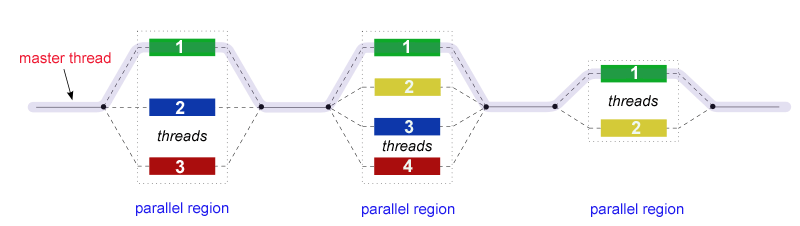
\includegraphics[width=\linewidth]{imagenes/fork-join.png}
	\caption{Modelo \textit{fork-join} \cite{Lawrence2019}}
	\label{fig:fork-join}
\end{figure}

Surge en 1997, cuando Intel impulsa la creación del OpenMP Architecture Review Board (ARB), un consorcio formado por fabricantes de hardware y software (Intel, IBM, AMD, HP, Nvidia, Oracle, entre otros) con el objetivo de definir un estándar común para paralelismo en memoria compartida. La última versión de OpenMP, la 6.0, data de 2024.

OpenMP aprovecha el paralelismo mediante \textit{multithreading}. El funcionamiento es relativamente simple, el programa comienza con un comportamiento secuencial y un hilo maestro. Cuando este hilo se encuentra una región paralela específica con \texttt{\#pragma omp parallel}, se crea un equipo de hilos \cite{ARB2024}. Los hilos ejecutan el bloque paralelo de forma concurrente, y al finalizar, los hilos se unen y el control vuelve al maestro.

Podemos identificar varios elementos principales, el primero de los cuales sería las directivas de compilador, como \texttt{\#pragma omp parallel}, \texttt{\#pragma omp for}, o \texttt{\#pragma omp single}, y sus cláusulas como \texttt{schedule}, \texttt{shared}, o \texttt{default}. Otros elementos importantes son las funciones de biblioteca, como \texttt{omp\_set\_num\_threads()} o \texttt{omp\_get\_wtime()}, y las variables de entorno, como \texttt{OMP\_NUM\_THREADS}, \texttt{OMP\_SCHEDULE}, o \texttt{OMP\_DYNAMIC}. \cite{ARB2024} 

Como hemos comentado, OpenMP opera sobre un modelo de memoria compartida en la que todos los hilos ven el mismo espacio de direcciones de memoria, en el que las variables pueden ser visibles por todos los hilos ($shared$), o cada hilo tiene su propia copia de una variable ($private$). Este modelo evita la necesidad de comunicación explícita entre procesos (como en MPI)\cite{Jin2024}, simplificando el desarrollo. 

\section{CUDA}

\textbf{CUDA}, siglas de \textit{Compute Unified Device Architecture} es una plataforma de computación paralela y un conjunto de APIs desarrollado por NVIDIA para ejecutar código general en sus GPUs. Incluye, entre otros, un modelo de programación a partir de C y C++; herramientas de compilación que generan código tanto para CPU como para GPU; un entorno de ejecución y una API para gestionar memoria, lanzamientos de kernels, streams; y librerías construidas sobre el propio modelo \cite{Kirk2010}. La idea principal es permitir que el programador trate a la GPU como un dispositivo de \textbf{cómputo masivamente paralelo}.

A modo de referencia, los primeros trabajos en los que se utiliza una GPU para cómputo general aparecen a principios de los 2000, en 2004 se crea internamente CUDA, y se lanza oficialmente en 2007. Desde entonces, la evolución de CUDA ha ido ligada a la evolución propia de las GPUs de NVIDIA, manteniendo el modelo de ejecución \textbf{SIMT}\textit{(Single Instruction, Multiple Threads)} y añadiendo unidades especializadas como \textit{Tensor Cores}, \textit{Ray Trancing Cores}, o el mecanismo del \textit{Transformer Engine} \cite{NVIDIA2026}.

CUDA implementa un modelo SIMT, en el cual el programador define una función denominada kernel que describe el código de un hilo, que se lanza desde la GPU y se ejecuta de forma concurrente en la GPU usando múltiples hilos. Los hilos se agrupan en bloques, que son arrays tridimensionales de hilos; y los bloques a su vez se agrupan como una grid, array tridimensional de bloques. Cada bloque se ejecuta en un \textit{Streaming Multiprocessor}, dentro del cual los hilos se agrupan en \textbf{warps de 32 hilos} que se ejecutan físicamente en paralelo utilizando cores del multiprocesador. \cite{Kirk2010} El warp de hilos es, por tanto, la unidad de ejecución con la que trabajamos.

\textbf{\Huge AÑADIR FIGURA DIAPOSITIVAS PROFESOR}

Cuando se programa con CUDA se ha de tener en mente que se puede acceder a varias \textbf{memorias diferentes}, cada una con su propia latencia y ancho de banda, y entre ellas nos encontramos a los \textbf{registros}, que son la memoria de los hilos individuales, y la más rápida de todas; pasando por la \textbf{memoria compartida} (\texttt{\_\_shared\_\_}), que usan los bloques; la \textbf{memoria de constantes} (\texttt{\_\_constant\_\_}), que es de solo lectura, y va cacheada; y la \textbf{memoria global}, que se aloja en la VRAM de la GPU, que es la que se utiliza para almacenar grandes estructuras de datos. \cite{Farber2011}

\begin{figure}[H]
	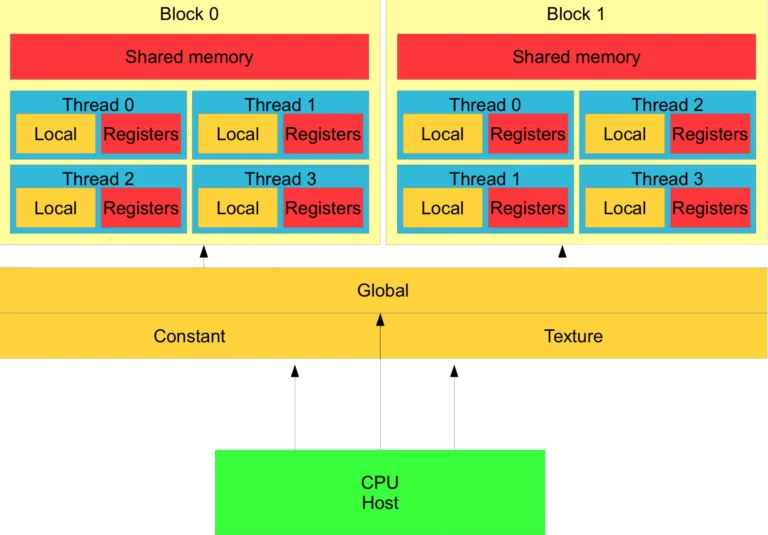
\includegraphics[width=\linewidth]{imagenes/CUDA-Memory-Hierarchy.png}
	\caption{Jerarquía de memorias en CUDA \cite{Beard2020} }
	\label{fig:CUDA-Memory-Hierarchy}
\end{figure}

El rendimiento de la memoria dependerá del buen hacer del programador, que será el encargado de buscar la coalescencia en los accesos a memoria global, del uso de  para reutilizar datos, de que evite la divergencia de los warps, y de que se encargue de controlar los warps activos. 

La \textbf{máxima coalescencia} ocurre cuando los 32 hilos de un warp acceden a direcciones de memoria que caen dentro del mínimo número de segmentos continuos necesarios para almacenar dichos datos \cite{Kirk2010}. Esto permite que la GPU atienda todos esos accesos el mínimo número de trabsacciones, lo cual implica la mayor eficiencia en el kernel al acceder a esos datos en memoria VRAM. 

Por otro lado, la \textbf{divergencia de warps} ocurre cuando los hilos de un mismo warp toman caminos distintos en una rama condicional. Como el warp ejecuta las instrucciones en modo SIMT, si los hilos divergen, el hardware debe serializar las rutas \cite{Farber2011}. Esto quiere decir que si los hilos se encuentran frente a un bloque if/else, lo que va a pasar es que el bloque if será ejecutado por los hilos que cumplan la condición, y el resto de hilos se quedarán en stand-by. A continuación, el resto de los hilos ejecutará el bloque else mientras los primeros se quedan esperando, y luego se combinarán los resultados.

Hay un matiz importante a tener en cuenta a la hora de describir la implementación CUDA, y es que lo que veremos a continuación serán funciones kernels, y no métodos de clase como vimos en el capítulo anterior. Una forma de verlo es que tendremos clases (como \texttt{Metodo}), y éstas tendrán sus funciones miembro que accederemos de forma normal con un objeto de la clase. Por otro lado tendremos las funciones kernel, que podrán ser llamados o no desde los métodos de las clases, y será donde ocurra el paralelismo de CUDA.

Aunque tengamos los kernel implementados en los archivos \texttt{.cu} de las clases, formalmente no son parte de ellas, son métodos globales que pueden ser llamados desde cualquier parte del código.

Como antes mencionamos, los kernel CUDA funcionan con \textbf{grids, bloques, y hebras}, y estos elementos interaccionan entre sí. Cuando llamamos a un kernel se crea una grid, que no es más que un conjunto de bloques con un tamaño predeterminado. Esta grid podrá tener una, dos, o tres dimensiones, y en cualquiera de los casos contendrá un número determinado de bloques. Estos bloques a su vez también tendrán de una a tres dimensiones y contendrán a las hebras, que serán con las que nosotros trabajaremos, indicando a cada hebra qué hacer dentro del kernel.

Aquí podemos ver un ejemplo ilustrativo en el que un kernel particular es llamado y crea una grid bidimensional de bloques, y a su vez los bloques por dentro son tridimensionales.

\begin{figure}[H]
	\centering
	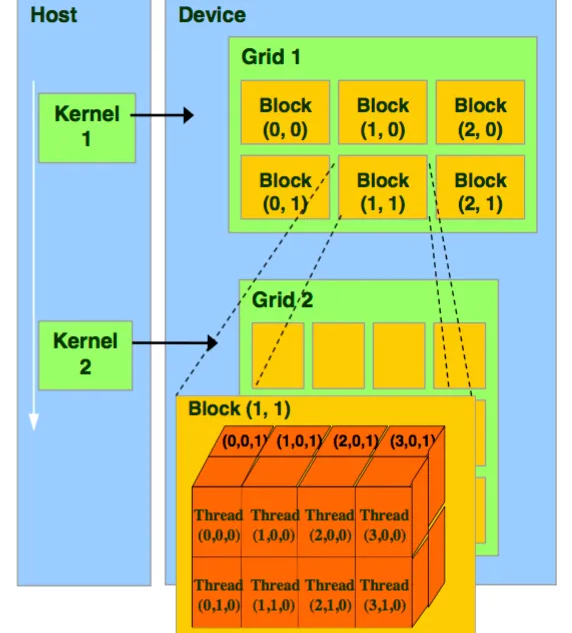
\includegraphics[width=0.65\linewidth]{imagenes/CUDA-blocks-grids.png}
	\caption{Grids y bloques CUDA \cite{Casas2024}}
	\label{fig:CUDA-blocks-grids}
\end{figure}

Como primer ejemplo para ilustrar el modelo, podemos tomar una función auxiliar de la clase \texttt{Metodo} como la que ya vimos implementada en OpenMP (algoritmo \ref{alg:VectorCopia-OMP}), y transformarla al paradigma de programación de CUDA. 

\begin{algorithm}[H]
	\begin{algorithmic}
		\State $ i \gets \text{blockDim.x} \cdot \text{blockIdx.x + threadIdx.x} $
		\If{ $ i < N $ }
		\State $ Y[i] \gets X[i]$
		\EndIf
	\end{algorithmic}
	\caption{Kernel de vectorCopia}
	\label{alg:Vector-Copia-CUDA}
\end{algorithm}

Por un lado, como podemos ver en la primera línea, se calcula un valor $i$ que es igual a una multiplicación y una suma. Identificando a esos 3 elementos tenemos primero a \texttt{blockDim.x}, que es un valor igual al tamaño de la dimensión X del bloque al que pertenezca cada thread particular. Luego, \texttt{blockIdx.x} designa al bloque individual que contenga cada thread que ejecute el kernel, y de igual manera \texttt{threadIdx.x} será el identificador individual de cada thread dentro de su bloque. Combinando los 3 generamos un identificador único para cada uno de los threads que genere el todo el grid.

Por otro lado, se hace la comprobación de que el identificador del thread es menor que el tamaño de los vectores para evitar posibles accesos erróneos a memoria. Esto ha de hacerse ya que, si tenemos un tamaño de problema N, se generará un grid con tantos bloques de tamaño \texttt{blockDim.x} como para que el total de hebras sea siempre mayor o igual a N. Dicho de otra forma, con un tamaño de bloque de 256, y un tamaño de problema de 1000, se generaría una grid con 4 bloques (y por tanto 1024 hebras), y las últimas 24 no trabajarían. % Capitulo 2.7 y 2.8
	\creaCapitulo{OpenMP}

OpenMP es un modelo de programación paralela para arquitecturas de memoria compartida, diseñado para proporcionar una interfaz portable, escalable y de alto nivel que permita explotar el paralelismo en CPUs multinúcleo sin recurrir a APIs de hilos de bajo nivel. Su diseño se basa en directivas de compilador, rutinas de biblioteca y variables de entorno, y sigue el modelo de ejecución \textit{fork–join}, donde un hilo maestro crea y sincroniza equipos de hilos que ejecutan regiones paralelas. \cite{Jin2024}

Surge en 1997, cuando Intel impulsa la creación del OpenMP Architecture Review Board (ARB), un consorcio formado por fabricantes de hardware y software (Intel, IBM, AMD, HP, Nvidia, Oracle, entre otros) con el objetivo de definir un estándar común para paralelismo en memoria compartida. La última versión de OpenMP, la 6.0, data de 2024.

OpenMP implementa paralelismo mediante \textit{multithreading}. El funcionamiento es relativamente simple, el programa comienza con un comportamiento secuencial y un hilo maestro. Cuando este hilo se encuentra una región paralela con \textit{\#pragma omp parallel}, se crea un equipo de hilos \cite{ARB2024}. Los hilos ejecutan el bloque paralelo de forma concurrente, y al finalizar, los hilos se unen y el control vuelve al maestro.

Podemos identificar se compone de varios elementos principales, el primero de los cuales sería las directivas de compilador, como \textit{\#pragma omp parallel}, \textit{\#pragma omp for}, o \textit{\#pragma omp single}, y sus cláusulas como \textit{schedule}, \textit{shared}, o \textit{default}. Otros elementos importantes son las funciones de biblioteca, como \textit{omp\_set\_num\_threads()} o \textit{omp\_get\_wtime()}, y las variables de entorno, como \textit{OMP\_NUM\_THREADS}, \textit{OMP\_SCHEDULE}, o \textit{OMP\_DYNAMIC}. \cite{ARB2024} 

Como hemos comentado, OpenMP opera sobre un modelo de memoria compartida en la que todos los hilos ven el mismo espacio de direcciones, en el que las variables pueden ser visibles por todos los hilos ($shared$), o cada hilo tiene su propia copia ($private$). Este modelo evita la necesidad de comunicación explícita entre procesos (como en MPI), simplificando el desarrollo. \cite{Jin2024}

\creaSeccion{Implementación Secuencial}

Tomaremos como punto de partida la implementación secuencial de los problemas \cite{Mantas2024}, de la cual ya disponemos.

\begin{figure}[H]
	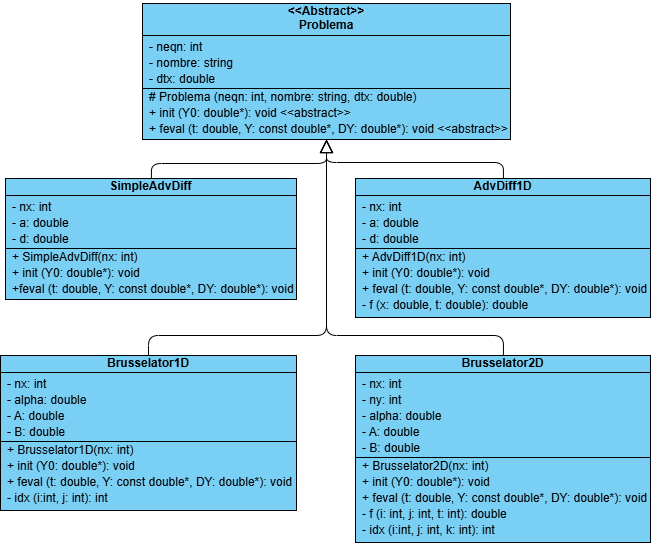
\includegraphics[width=\linewidth]{imagenes/OMP-Diagrama-Problemas.png}
	\caption{Diagrama de Clases de los problemas OMP}
	\label{fig:OMP-Diagrama-Problemas}
\end{figure}

Como comentamos anteriormente, no nos centraremos en la resolución de los problemas \textit{per se}, puesto que ésta se nos da ya hecha y corregida, sino que nuestros esfuerzos irán en implementar los métodos de resolución en ambas formas de paralelismo, y buscar la máxima eficiencia. Para facilitar la implementación y la cohesión del código, definimos una clase abstracta \textit{Problema} de la cual heredarán los cuatro problemas.

El siguiente paso, por tanto, será realizar una implementación secuencial de los métodos, partiendo de los algoritmos que previamente hemos comentado, Runge-Kutta, Adams-Bashford, y Adamd-Bashford-Moulton, a saber, algoritmos \ref{alg:RungeKutta4}, \ref{alg:AdamsBashford}, y \ref{alg:AdamsBashfordMoulton}, respectivamente. El lenguaje elegido será C++, para luego poder añadir la parte de OpenMP o CUDA.

\begin{figure}[H]
	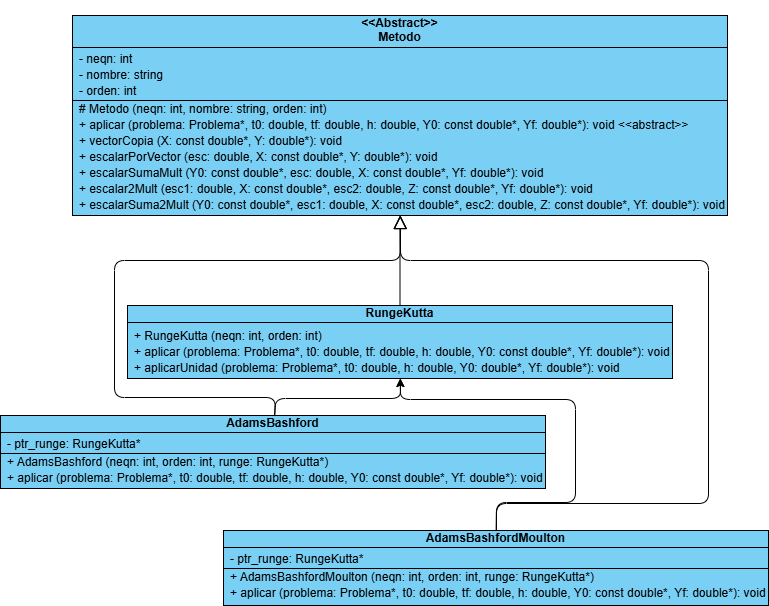
\includegraphics[width=\linewidth]{imagenes/OMP-Diagrama-Metodos.png}
	\caption{Diagrama de Clases de los métodos OMP}
	\label{fig:OMP-Diagrama-Metodos}
\end{figure}

El planteamiento que se hace con los métodos es similar al de los problemas, una clase abstracta padre de la cual puedan heredar los métodos. Además, en la clase padre \textit{Metodo} hemos implementado diversas funciones auxiliares que nos van a facilitar el trabajar con vectores. Con este diseño, a través de la herencia y el polimorfismo, podríamos aumentar el alcance de nuestro proyecto añadiendo nuevos métodos o más problemas sin dificultad ninguna.

Ahora que tenemos una primera maqueta funcional (aunque poco eficiente), podremos comenzar con el trabajo en paralelo. De cara a nuestro proyecto, lo primero que debemos tener en cuenta es que no podemos simplemente paralelizar el bucle principal con el que trabajamos (e.g. el bucle while en el algoritmo \ref{alg:AdamsBashford}) porque cada iteración necesita de la anterior para calcular el siguiente paso. Deberemos buscar por tanto otras formas de atacar el problema. En el caso de OpenMP hemos planteado dos formas, paralelismo por operaciones, y por componentes.

\creaSeccion{Paralelismo por Operaciones}

En esta estrategia buscamos que cada función paralelice su propio trabajo. Eso quiere decir que cada operación vectorial, como el \textit{feval()}, o \textit{escalarPorVector}, tiene su propio \textit{\#pragma omp parallel}, crea un equipo de hilos, reparte el trabajo, y lo sincroniza.

De forma simplificada, veamos un ejemplo de Adams-Bashford 4:

\begin{algorithm}[H]
	\begin{algorithmic}
		\State $ Y_{n0} \gets Y_0 $
		\State $ Y_n \gets arranqueRK4(Y_{n-1})$ \Comment{$ n = \{1, 2, 3\} $}
		\State $ F_n \gets feval(t_n\text{, }Y_n)$ \Comment{$ n = \{0, 1, 2, 3\} $}
		\For{ $ t_n \text{=} t_0 \text{+} 3h \text{; }t_n < t_f\text{; }t_n \text{+=}h $ }
			\State $ escalar2Mult(37.0\text{, }F_{n1}\text{, -}9.0\text{, }F_{n0}\text{, }Y_{aux}) $
			\State $ escalarSuma2Mult( Y_{aux}\text{, }55.0\text{, }F_{n3}\text{, -}59.0\text{, }F_{n2}\text{, }Y_{aux} ) $
			\State $ escalarSumaMult( Y_{n3}\text{, }h/24.0\text{, }Y_{aux}\text{, }Y_{n4} ) $
			\State $ F_{n4} \gets feval(t_n+h\text{, }Y_{n4}) $
			
			\State $ swap(Y_{n4}\text{, }Y_{n3}) $
			\State $ swap(F_n\text{, }F_{n-1}) $ \Comment{$ n = \{1, 2, 3, 4\} $}
		\EndFor
		\State $Y_f \gets Y_{n3}$
	\end{algorithmic}
	\caption{Implementación de AB4 con Paralelismo por Operaciones}
	\label{alg:AB4ParalelismoOperaciones}
\end{algorithm}

Como podemos ver, para hacer el cálculo propio de Adams-Bashford de orden 4 (ecuación \ref{eq:AdamsBashford4}) la hemos divido en 3 partes utilizando las funciones auxiliares de la clase abstracta \textit{Metodo} de las que ya disponíamos. Dentro de cada una de ellas se creará el grupo de hilos, se repartirá el trabajo (cada hilo tendrá un "trozo" de vector sobre el que trabajar), y una vez finalicen se sincronizará para retornar a la función principal. Por ejemplo, \textit{vectorCopia()}:
\begin{algorithm}[H]
	\begin{algorithmic}
		\State \verb|#pragma omp parallel for schedule(static)|
		\For{ $ i \text{=} 0 \text{; }i < neqn\text{; }\text{++}i $ }
			\State $ Y[i] \gets X[i] $
		\EndFor
		
	\end{algorithmic}
	\caption{Implementación de Función Auxiliar vectorCopia}
	\label{alg:VectorCopia-OMP}
\end{algorithm}

Esta estrategia trae consigo ventajas como la modularidad, ya que cada operación vectorial es independiente y autocontenida, lo cual facilita la depuración y la legibilidad del código.

El principal punto negativo de esta estrategia es que trae consigo un \textit{overhead} alto, ya que cada función tiene una barrera implícita al acabar un \textit{parallel for}, en cada iteración del bucle hay varias llamadas a funciones, y el bucle itera un elevado número de veces. Esto equivale a más paradas de las que serían deseadas, además de que los hilos entran y salen de regiones paralelas constantemente.

\creaSeccion{Paralelismo por Componentes}

Frente al paralelismo de operaciones, tenemos el paralelismo por componentes (o por elementos), en el que sólo tenemos una gran región \textit{parallel} dentro de la cual ocurre todo el paralelismo, y cada hebra calcula su parte de los vectores.

Esto quiere decir que se creará un único equipo de hilos al entrar en el \textit{parallel}, y todos los hilos permanecerán activos e iterarán en el bucle, paso a paso. Dentro del bucle iterativo, habrá diversos \textit{\#pragma omp for} que repartirán los índices entre los hilos. Esto además nos permitirá reducir las barreras de sincronización. Para poder comparar con la anterior implementación \ref{alg:AB4ParalelismoOperaciones}, describimos el mismo algoritmo (\ref{eq:AdamsBashford4}) pero con esta estrategia:

\begin{algorithm}[H]
	\begin{algorithmic}
		\State $ Y_{n0} \gets Y_0 $
		\State $ Y_n \gets arranqueRK4(Y_{n-1})$ \Comment{$ n = \{1, 2, 3\} $}
		\State \verb|#pragma omp parallel for schedule(static)|
		\For{ $ i \text{=} 0 \text{; }i < neqn\text{; }\text{++}i $ }
			\State $ F_n[i] \gets feval\_i(t_n\text{, }Y_n\text{, }i)$ \Comment{$ n = \{0, 1, 2, 3\} $}
		\EndFor
		
		\State \verb|#pragma omp parallel|
		\For{ $ t_n \text{=} t_0 \text{+} 3h \text{; }t_n < t_f\text{; }t_n \text{+=}h $ }
			\State \verb|#pragma omp for schedule(static)|
			\For{ $ i \text{=} 0 \text{; }i < neqn\text{; }\text{++}i $ }
				\State $ Y_4[i] = Y_3[i] + h/24 * ( 55F_3[i] - 59F_2[i] + 37F_1[i] -9F_0[i]) $
			\EndFor
			\State \verb|#pragma omp for schedule(static)|
			\For{ $ i \text{=} 0 \text{; }i < neqn\text{; }\text{++}i $ }
				\State $ F_4[i] \gets feval\_i(t_n+h\text{, }Y_4\text{, }i)$
			\EndFor
			\State \verb|#pragma omp single|
			\State $ swap(Y_{n4}\text{, }Y_{n3}) $
			\State $ swap(F_n\text{, }F_{n-1}) $ \Comment{$ n = \{1, 2, 3, 4\} $}
		\EndFor
		\State $Y_f \gets Y_{n3}$
	\end{algorithmic}
	\caption{Implementación de AB4 con Paralelismo por Componentes}
	\label{alg:AB4ParalelismoComponentes}
\end{algorithm}

La idea principal detrás de esta estrategia es reducir el \textit{overhead} provocado por tener demasiadas barreras de sincronización, y mejorar el uso de la caché. Para mejorar la implementación hacemos uso de directivas como \textit{schedule (static)}, con la que indicamos cómo deben repartirse las iteraciones entre los hilos. En este caso, se divide el rango de iteraciones en bloques contiguos y de tamaño fijo, y se asigna cada bloque a un hilo antes de empezar la ejecución del bucle. Esto es práctico cuando sabemos de antemano que todas las iteraciones van a costar lo mismo, y no va haber ramas pesadas o irregulares.

Algunas de las desventajas que tendremos es que el código es más complejo, pues no se puede reutilizar el \textit{feval()} secuencial (que sí lo aprovechábamos en el paralelismo por operaciones), sino que hay que hacer una versión específica para los componentes. De igual manera, no se pueden utilizar las funciones auxiliares, porque están diseñadas para tratar los vectores completos, no elementos individuales.

\creaSeccion{Mediciones}

Ante la pregunta de qué estrategia es mejor, la respuesta sería, como casi siempre en informática, que depende.

En un primer planteamiento, parece que el paralelismo por componentes debería ser mejor. Reduce la creación y destrucción repetitiva de las hebras, y reduce las barreras de sincronización.

Un matiz importante que debemos hacer es que, aunque hablemos de creación y destrucción de hilos iterativa, no siempre ha de ocurrir así. Es cierto que, de forma lógica, el modelo \textit{fork-join} de OpenMP describe de esa forma el comportamiento de los hilos; se crean, se usan, se destruyen. \cite{Jin2024} Sin embargo, esto no siempre ocurre así (ya que sería muy costoso).

Existe un concepto llamado \textit{thread pooling}, que describe que el entorno de ejecución podrá devolver los hilos a la \textit{pool} en lugar de destruirlos, y así ahorrarse crearlos posteriormente. \cite{Barlas2023} Esto eliminaría la principal desventaja del paralelismo por operaciones. 

De forma análoga, el \textit{runtime} no siempre mantiene los hilos activos (como pudiera parecer), aunque no haya finalizado el bloque \textit{parallel}, ya que si el trabajo dentro de cada bloque \textit{omp for} es pequeño, el compilador puede decidir dormir los hilos para ahorrar energía. Esto puede provocar pérdida de tiempo al tener que despertar los hilos, y latencias de sincronización más altas.

Otro dato a tener en cuenta, es que en el planteamiento de nuestros problemas, las llamadas a \textit{feval\_i()} son muy baratas, y el trabajo por iteración es pequeño, mientras que \textit{feval()} es más pesado, y en cierta forma se amortiza el \textit{overhead} al hacerse  una única llamada en lugar de \textit{neqn} llamadas.

Podemos comenzar, por ejemplo, comparando los tiempos al resolver el problema \textit{Brusselator1D} con 100.000 ecuaciones.
\begin{table}[H]
	\begin{center}
		\begin{tabular}{| c | c | c | c |}
			\hline
			\textbf{Solver} & \textbf{Hebras} & \textbf{Estrategia} & \textbf{T (s)} \\
			\hline
			
			% ---------------- RUNGE KUTTA ----------------
			\multirow{6}{*}{Runge-Kutta}
			& \multirow{2}{*}{1}  & OMP Componentes   & 2501.84 \\
			\cline{3-4}
			&                     & OMP Operaciones & 1544.87 \\
			\cline{2-4}
			& \multirow{2}{*}{4}  & OMP Componentes   & 670.504 \\
			\cline{3-4}
			&                     & OMP Operaciones & 371.93 \\
			\cline{2-4}
			& \multirow{2}{*}{16} & OMP Componentes   & 197.065 \\
			\cline{3-4}
			&                     & OMP Operaciones & 180.327 \\
			\hline
			
			% ---------------- ADAMS BASHFORD ----------------
			\multirow{6}{*}{Adams-Bashford}
			& \multirow{2}{*}{1}  & OMP Componentes   & 707.634 \\
			\cline{3-4}
			&                     & OMP Operaciones & 556.051 \\
			\cline{2-4}
			& \multirow{2}{*}{4}  & OMP Componentes   & 179.559 \\
			\cline{3-4}
			&                     & OMP Operaciones & 130.993 \\
			\cline{2-4}
			& \multirow{2}{*}{16} & OMP Componentes   & 56.5174 \\
			\cline{3-4}
			&                     & OMP Operaciones & 66.1485 \\
			\cline{3-4}
			\hline
			
			% ---------------- ADAMS BASHFORD MOULTON ----------------
			\multirow{6}{*}{Adams-Bashford-Moulton}
			& \multirow{2}{*}{1}  & OMP Componentes   & 2914.04 \\
			\cline{3-4}
			&                     & OMP Operaciones & 1772.73 \\
			
			\cline{2-4}
			& \multirow{2}{*}{4}  & OMP Componentes   & 785.555 \\
			\cline{3-4}
			&                     & OMP Operaciones & 438.018 \\
			
			\cline{2-4}
			& \multirow{2}{*}{16} & OMP Componentes   & 237.236 \\
			\cline{3-4}
			&                     & OMP Operaciones & 219.918 \\
			
			\hline
			
		\end{tabular}
		\caption{Tiempos de Brusselator1D con 100000 ecuaciones}
		\label{tab:Brusselator1D-100K}
	\end{center}
\end{table}

\begin{figure}[H]
	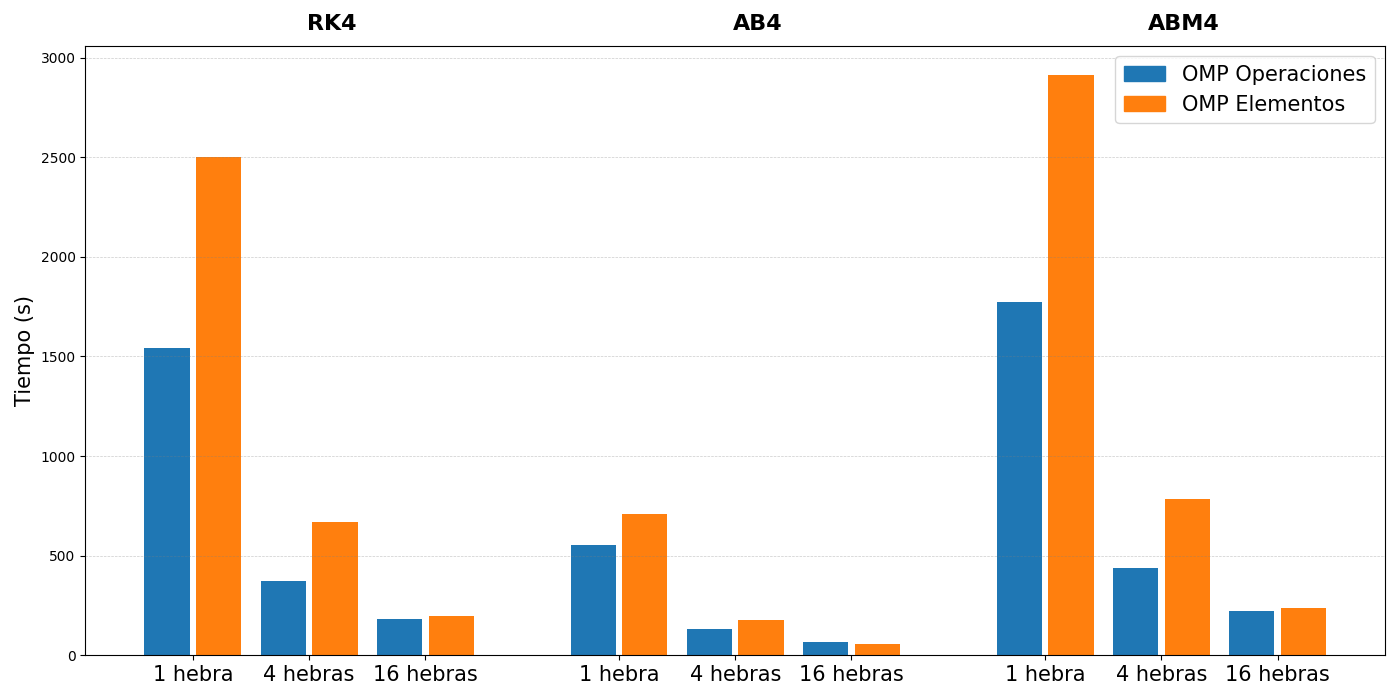
\includegraphics[width=\linewidth]{imagenes/Brusselator1D-100K.png}
	\caption{Brusselator1D 100.000 ecuaciones}
	\label{fig:Brusselator1D-100K}
\end{figure}

Como podemos ver, hay una mejora sustancial del tiempo al pasar de 1 a 4 y a 16 hebras, con ambas estrategias de paralelismo, y con los 3 métodos numéricos. Además, se aprecia que la resolución con Adams-Bashford es más rápida que Runge-Kutta, ya que es más directa y no requiere de los pasos intermedios (K1, K2, K3, K4), y también es mucho más veloz que el predictor-corrector Adams-Bashford-Moulton, ya que éste último llama a Adams-Bashford dentro de su bucle de ejecución. Además, podemos ver que para este tipo y tamaño de problema, el paralelismo por operaciones es más eficiente para 4 hebras, pero ambos se equiparan cuando se alcanzan las 16.

Podemos probar por ejemplo, con el problema más complejo (\textit{Brusselator2D}), y el método que más tarda (\textit{ABM4}), y podemos comparar la evolución del tiempo conforme aumenta el tamaño del problema, a saber, con un número de ecuaciones igual a 45000, 80000 y 125000.

\begin{table}[H]
	\begin{center}
		\begin{tabular}{| c | c | c | c | c | c |}
			\hline
			\textbf{neqn} & \textbf{Hebras} & \textbf{Estrategia} & \textbf{T (s)} & \textbf{Speedup} & \textbf{Eficiencia} \\
			\hline
			
			% ---------------- 45000 ----------------
			\multirow{6}{*}{45000}
			& \multirow{2}{*}{1}  & Operaciones & 976.061 & \multirow{2}{*}{1} & \multirow{2}{*}{100} \\
			\cline{3-4}
			&                     & Componentes & 2151.79 &                   &                    \\
			\cline{2-6}
			& \multirow{2}{*}{4}  & Operaciones & 263.081 & 3.710115896 & 92.7528974 \\
			\cline{3-6}
			&                     & Componentes & 569.693 & 3.777104511 & 94.4276128 \\
			\cline{2-6}
			& \multirow{2}{*}{16} & Operaciones & 180.662 & 5.402691213 & 33.7668201 \\
			\cline{3-6}
			&                     & Componentes & 206.744 & 10.40799249 & 65.0499531 \\
			\hline
			
			% ---------------- 80000 ----------------
			\multirow{6}{*}{80000}
			& \multirow{2}{*}{1}  & Operaciones & 1825.86 & \multirow{2}{*}{1} & \multirow{2}{*}{100} \\
			\cline{3-4}
			&                     & Componentes & 3970.37 &                   &                    \\
			\cline{2-6}
			& \multirow{2}{*}{4}  & Operaciones & 466.282 & 3.915784868 & 97.8946217 \\
			\cline{3-6}
			&                     & Componentes & 1049.35 & 3.78364702 & 94.5911755 \\
			\cline{2-6}
			& \multirow{2}{*}{16} & Operaciones & 214.67 & 8.505426934 & 53.1589183 \\
			\cline{3-6}
			&                     & Componentes & 331.809 & 11.96582974 & 74.7864359 \\
			\hline
			
			% ---------------- 125000 ----------------
			\multirow{6}{*}{125000}
			& \multirow{2}{*}{1}  & Operaciones & 2692.79 & \multirow{2}{*}{1} & \multirow{2}{*}{100} \\
			\cline{3-4}
			&                     & Componentes & 5982.94 &                   &                    \\
			\cline{2-6}
			& \multirow{2}{*}{4}  & Operaciones & 675.123 & 3.988591708 & 99.7147927 \\
			\cline{3-6}
			&                     & Componentes & 1593.61 & 3.754331361 & 93.8582840 \\
			\cline{2-6}
			& \multirow{2}{*}{16} & Operaciones & 264.402 & 10.18445398 & 63.6528373 \\
			\cline{3-6}
			&                     & Componentes & 445.081 & 13.44236218 & 84.0147636 \\
			\hline
			
		\end{tabular}
		\caption{Brusselator2D con ABM4}
		\label{tab:Brusselator2D-ABM4}
	\end{center}
\end{table}

Para calcular el speedup y la eficiencia, hemos comparado los valores de mismo tamaño y estrategia, para que la comparación sea más justa. Más allá de lo obvio, que conforme aumenta el tamaño del problema, aumentan los tiempos, es cuanto menos destacable la variación en los speedups que se alcanzan en función del aumento de las hebras, en una estrategia y otra.

\begin{figure}[H]
	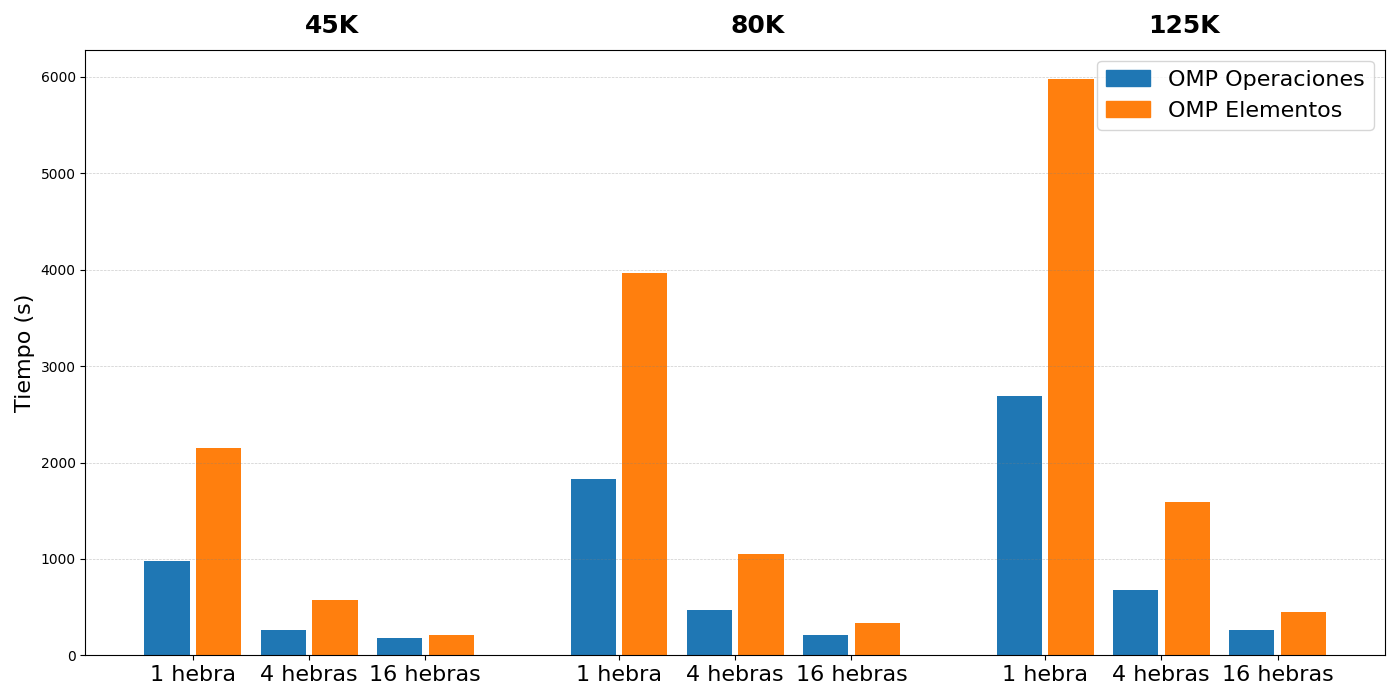
\includegraphics[width=\linewidth]{imagenes/Brusselator2D-ABM.png}
	\caption{ABM4 resolviendo Brusselator2D}
	\label{fig:Brusselator2D-ABM4}
\end{figure}

Partiendo de los mismos datos, pero tomando ahora solo el speedup y la eficiencia, y quedándonos con paralelismo de operaciones, tendríamos estas métricas:

\begin{figure}[H]
	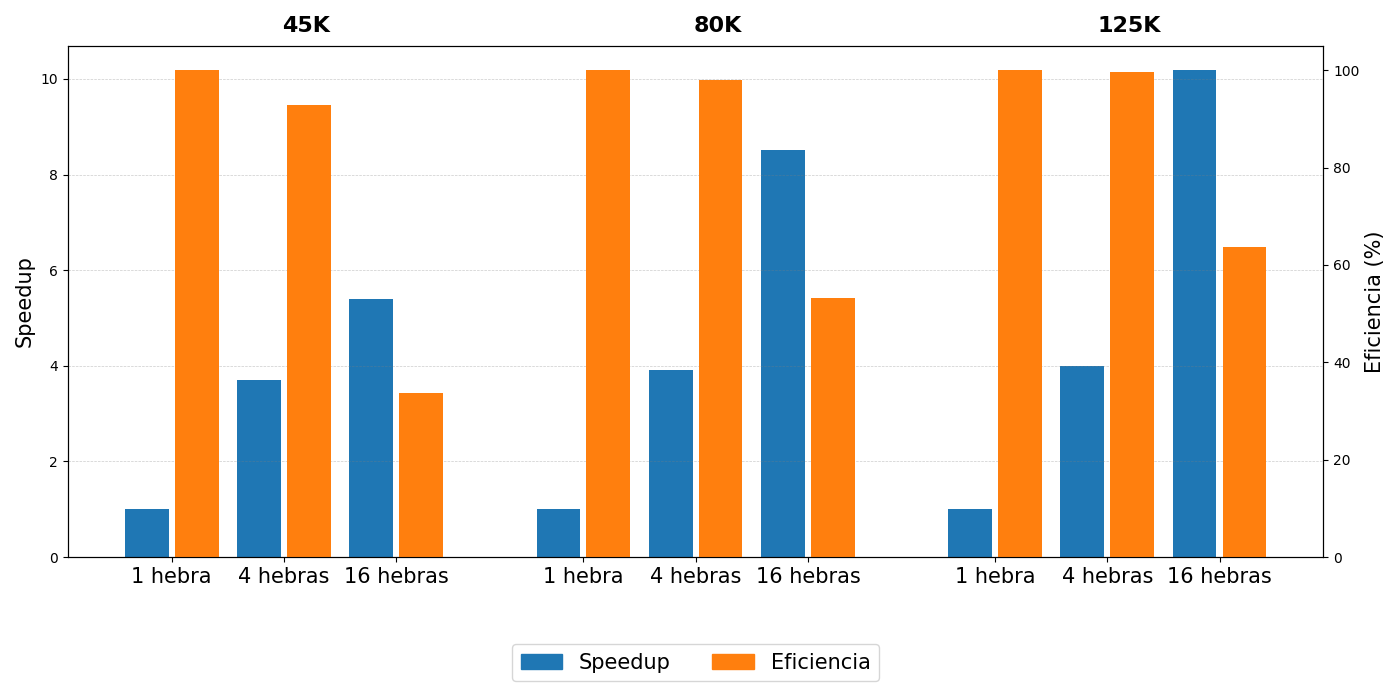
\includegraphics[width=\linewidth]{imagenes/OMP-Speedup-Eficiencia.png}
	\caption{Speedup y Eficiencia - ABM4 Brusselator2D}
	\label{fig:Spd-Eff-ABM4-Br2D}
\end{figure}

Tenemos la barras del speedup en azul y alineadas con el eje Y izquierdo, y en naranja y con el eje Y derecho la eficiencia en valores porcentuales. Obviamente, para 1 hebra siempre tendremos un speedup de 1, y una eficiencia de 100\%.

Más allá de eso, podemos ver varias ideas en juego a la vez. Si nos centramos en cualquiera de los 3 tamaños, podemos ver la Ley de Amdahl \cite{Amdahl1967} en funcionamiento; con un mismo tamaño de problema, conforme crece el número de hilos, aumenta el speedup pero disminuye la eficiencia, ya que siempre queda una parte secuencial que no se puede paralelizar.

Análogo a esto, si nos fijamos ahora en las columnas de la eficiencia, podemos ver que, para un mismo número de hebras, conforme aumenta el tamaño de problema, la eficiencia lo hace con él, pasando de un 33\%, a un 53\%, y a un 63\%, cuando observamos los datos relativos a las 16 hebras por ejemplo. Esto coincide con la ley de Gustafson \cite{Gustafson1988}, ya que al aumentar el tamaño del problema, crece la parte del programa que es paralelizable, y por lo tanto la eficiencia aumenta también. % Capitulo 3
	\creaCapitulo{CUDA}

CUDA, siglas de \textit{Compute Unified Device Architecture} es una plataforma de computación paralela y un conjunto de APIs desarrollado por NVIDIA para ejecutar código general en sus GPUs. Incluye, entre otros, un modelo de programación a partir de C y C++; un compilador (\textit{nvcc}) que genera código tanto para CPU como para GPU; un entorno de ejecución un una API para gestionar memoria, lanzamientos de kernels, streams; y librerías construidas sobre el propio modelo. \cite{Kirk2010} La idea principal es permitir que el programador trate a la GPU como un dispositivo de cómputo masivamente paralelo.

A modo de referencia, los primeros trabajos en los que se utiliza una GPU para cómputo general aparecen a principios de los 2000, en 2004 se crea internamente CUDA, y se lanza oficialmente en 2007. Desde entonces, la evolución de CUDA ha ido ligada a la evolución propia de las GPUs de NVIDIA, manteniendo el modelo \textit{SIMT} y añadiendo unidades especializadas como \textit{Tensor Cores}, \textit{RT Cores}, o el mecanismo del \textit{Transformer Engine}. \cite{NVIDIA2026}

CUDA implementa un modelo SIMT (Single Instruction, Multiple Threads), en el cual el programador define un kernel (función \textit{\_\_global\_\_}) que se ejecuta en muchos hilos. Los hilos se agrupan en bloques, y los bloques en una grid, y cada bloque se ejecuta en un \textit{Streaming Multiprocessor}, dentro del cual los hilos se agrupan en warps de 32 hilos. \cite{Kirk2010} El warp es por tanto la unidad de ejecución con la que trabajamos.

Cuando se trabaja con CUDA se ha de tener en mente que se puede acceder a varias memorias diferentes, cada una con su propia latencia y ancho de banda, y entre ellas nos encontramos a los registros, que son la memoria de los hilos individuales, y la más rápida de todas; pasando por la memoria compartida (\textit{\_\_shared\_\_}), que usan los bloques; la memoria constante(\textit{\_\_constant\_\_}), que es de solo lectura, y va cacheada; y la memoria global, que se aloja en la VRAM de la GPU. \cite{Farber2011}

El rendimiento de la memoria dependerá del buen hacer del programador, que será el encargado de buscar la coalescencia en los accesos a memoria global, del uso del \textit{shared memory} para reutilizar datos, de que evite la divergencia de los warps, y de que se encargue de controlar los warps activos. 

La coalescencia ocurre cuando los 32 hilos de un warp acceden a direcciones de memoria que caen dentro de un mismo segmento continuo. \cite{Kirk2010} Esto permite que la GPU atienda todos esos accesos con una sola transacción de memoria, lo cual implica una mayor eficiencia en el kernel. 

Por otro lado, la divergencia de warps ocurre cuando los hilos de un mismo warp toman caminos distintos en una rama condicional. Como el warp ejecuta las instrucciones en modo SIMT, si los hilos divergen, el hardware debe serializar las rutas. \cite{Farber2011} Esto quiere decir que si los hilos se encuentran frente a un bloque if/else, lo que va a pasar es que el bloque if será ejecutado por los hilos que cumplan la condición, y el resto de hilos se quedarán en stand-by. A continuación, el resto de los hilos ejecutará el bloque else mientras los primeros se quedan esperando, y luego se combinarán los resultados.  

Hay un matiz importante a tener en cuenta a la hora de hablar de implementaciones CUDA, y es que esto que veremos aquí serán kernels, y no métodos de clase como anteriormente. Una forma de verlo es que tendremos clases (como \textit{Metodo}), y éstas tendrán sus métodos que accederemos de forma normal con un objeto de la clase, y por otro lado tendremos los kernel, que podrán ser llamados o no desde los métodos de las clases, y será donde ocurra el paralelismo de CUDA.

Aunque tengamos los kernel implementados en los archivos \textit{.cu} de las clases, formalmente no son parte de ellas, son métodos globales que pueden ser llamados desde cualquier parte del código. Volviendo ahora a la implementación del kernel auxiliar que tenemos, hay varios conceptos a tener en cuenta.

Como antes mencionamos, los kernel CUDA funcionan con grids, bloques, y hebras, y estos elementos interaccionan entre sí. Cuando llamamos a un kernel se crea una grid, que no es más que un conjunto de bloques con un tamaño predeterminado. Esta grid podrá tener una, dos, o tres dimensiones, y en cualquiera de los casos contendrá un número determinado de bloques.

Estos bloques a su vez también tendrán de una a tres dimensiones y contendrán a las hebras, que serán con las que nosotros trabajaremos, indicando a cada hebra qué hacer dentro de los kernel. Si bien es cierto que aquí se aplicarán principalmente por defecto grids y bloques unidimensionales, salvo cuando se indique lo contrario.

Aquí podemos ver un ejemplo ilustrativo en el que un kernel particular es llamado y crea una grid bidimensional de bloques, y a su vez los bloques por dentro son tridimensionales.

\begin{figure}[H]
	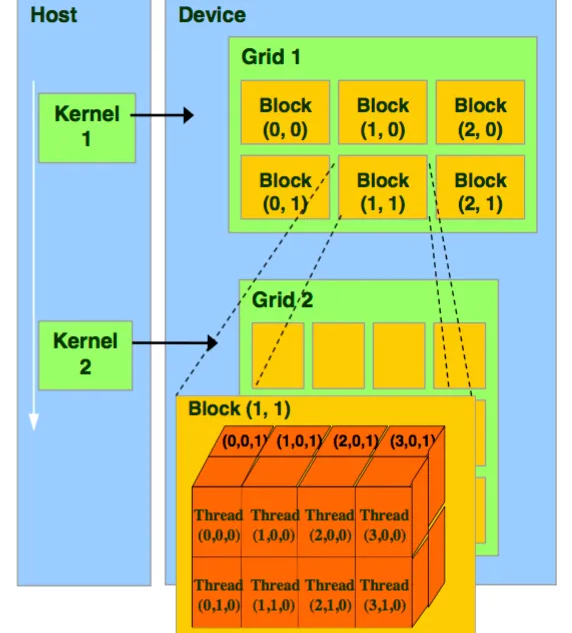
\includegraphics[width=\linewidth]{imagenes/CUDA-blocks-grids.png}
	\caption{Grids y bloques CUDA \cite{Casas2024} }
	\label{fig:CUDA-blocks-grids}
\end{figure}

Como primer ejemplo para ilustrar el modelo, podemos tomar una función auxiliar de la clase \textit{Metodo} como la que ya vimos implementada en OpenMP (algoritmo \ref{alg:VectorCopia-OMP}). En este caso veremos el kernel \textit{escalarPorVector()}. 

\begin{algorithm}[H]
	\begin{algorithmic}
		\State $ i \gets \text{blockDim.x} \cdot \text{blockIdx.x + threadIdx.x} $
		\If{ $ i < N $ }
			\State $ Y[i] \gets Y[i] + X[i] * esc $
		\EndIf
	\end{algorithmic}
	\caption{Kernel escalarPorVector}
	\label{alg:escalarPorVector}
\end{algorithm}

Por un lado, como podemos ver en la primera línea, se calcula un valor $i$ que es igual a una multiplicación y una suma. Identificando a esos 3 elementos tenemos primero a \textit{blockDim.x}, que es un valor igual al tamaño de la dimensión X del bloque al que pertenezca cada thread particular. Luego, \textit{blockIdx.x} designa al bloque individual que contenga cada thread que ejecute el kernel, y de igual manera \textit{threadIdx.x} será el identificador individual de cada thread dentro de su bloque. Combinando los 3 generamos un identificador único para cada uno de los threads que genere el grid.

Por otro lado, se hace la comprobación de que el identificador del thread es menor que el tamaño de los vectores para evitar posibles accesos erróneos a memoria. Esto ha de hacerse ya que, si tenemos un tamaño de problema N, se generará un grid con tantos bloques de tamaño \textit{blockDim.x} como para que el total de hebras sea siempre mayor o igual a N. Dicho de otra forma, con un tamaño de bloque de 256, y un tamaño de problema de 1000, se generaría una grid con 4 bloques (y por tanto 1024 hebras), y las últimas 24 no trabajarían. % Capitulo 4
	\chapter{Planificación}

A la hora de realizar un proyecto de esta magnitud, la planificación es de suma importancia, ya que a fin de cuentas es el pilar en el que se vertebra el proyecto, y que dicta qué se debe ir haciendo en cada momento. La planificación aquí expuesta ha permitido cumplir los objetivos inicialmente establecidos.
\begin{itemize}
	\item Abril: Definición del proyecto
	\begin{itemize}
		\item Identificación del tema a desarrollar
		\item Formulación de los objetivos
	\end{itemize}
	\item Mayo: Investigación
	\begin{itemize}
		\item Recopilación y revisión de libros y papers relevantes
		\item Búsqueda de información sobre las dos tecnologías de paralelización
	\end{itemize}
	\item Junio: Implementación de OpenMP
	\begin{itemize}
		\item Secuencial
		\item Paralelismo por operaciones
		\item Paralelismo por componentes
		\item Pruebas y validación del código
	\end{itemize}
	\item Julio: Implementación de CUDA
	\begin{itemize}
		\item Desarrollo de los kernels
		\item Kernels Graph
		\item Shuffles y grids
		\item Pruebas y validación del código
	\end{itemize}
	\item Agosto: Memoria del proyecto
	\begin{itemize}
		\item Mediciones temporales
		\item Análisis de los datos
		\item Redacción de la memoria
	\end{itemize}
	\item Septiembre: Entrega
	\begin{itemize}
		\item Últimas correcciones
		\item Presentación y defensa
	\end{itemize}
\end{itemize}

\begin{figure}[H]
	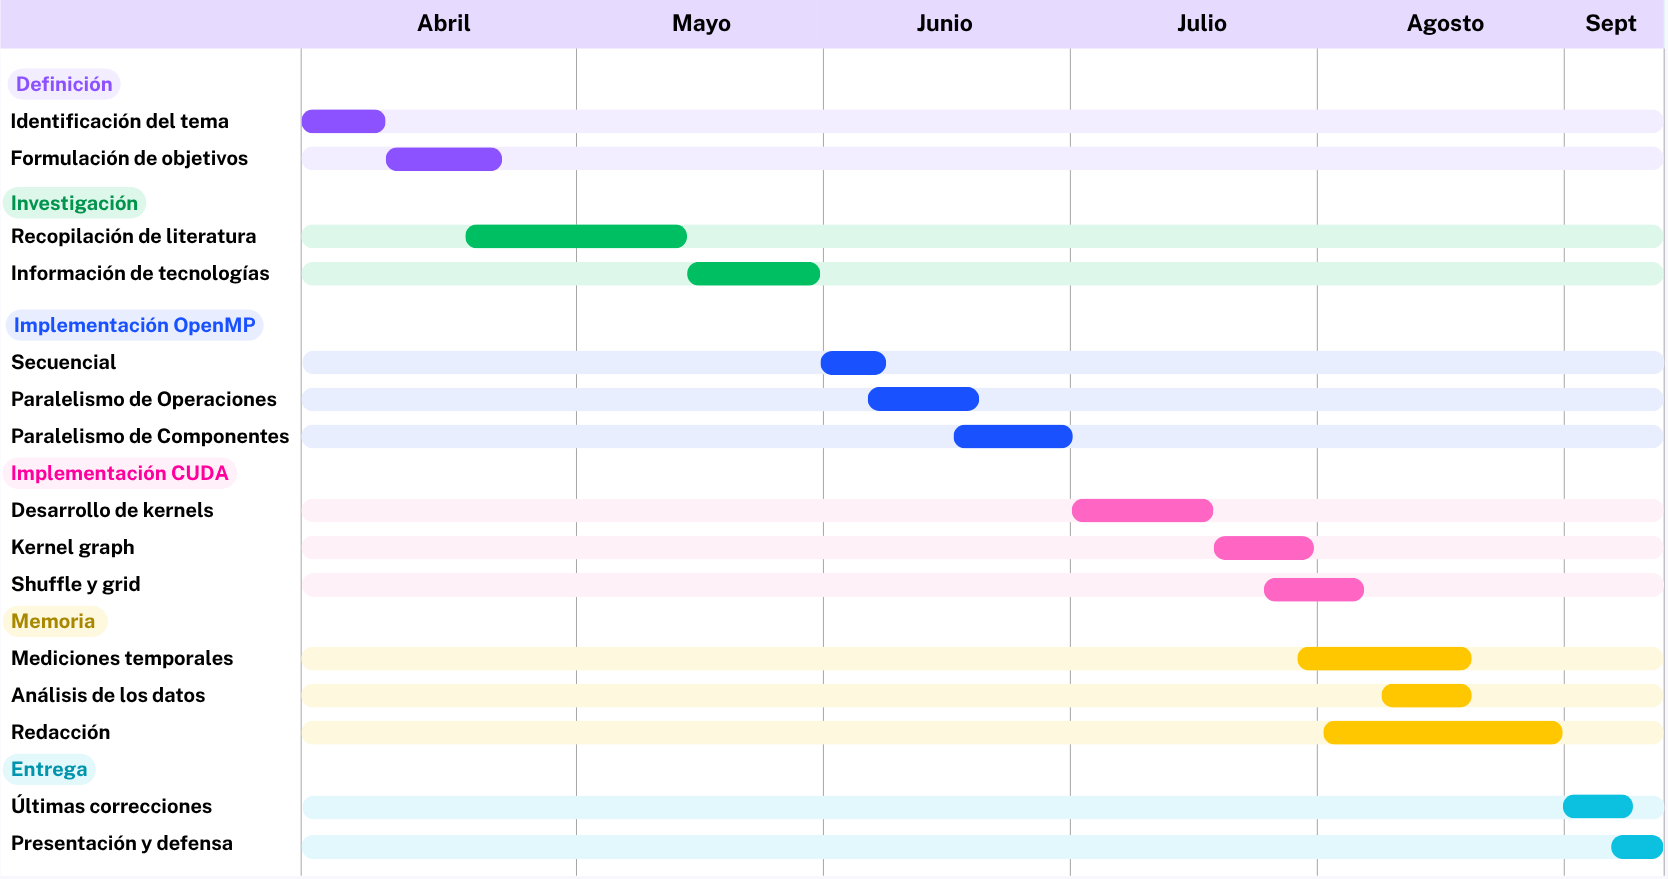
\includegraphics[width=\linewidth]{imagenes/Diagrama-Gantt.png}
	\caption{Diagrama de Gantt}
	\label{fig:Diagrama-Gantt}
\end{figure}

\chapter{Código fuente}

El código desarrollado, así como las diferentes partes que componen esta memoria se encuentran el el siguiente repositorio:

\url{https://github.com/PepeNavarro7/TFG}

GitHub es una plataforma online donde los desarrolladores almacenan, comparten y colaboran en proyectos de programación usando Git, que es un sistema de control de versiones distribuido, que sirve para guardar el historial de un proyecto, comparar versiones, volver atrás, trabajar en paralelo y fusionar cambios sin perder nada.

Para usar el proyecto, basta con descargar cualquiera de las dos carpetas del solver (OpenMP o CUDA), y ejecutar el Makefile siguiendo las intrucciones que vienen dentro del mismo, que permiten la ejecución de un solo test, o de una batería de ellos.

Para las mediciones que se muestran en el presente proyecto se utilizó ese mismo código fuente ejecutado desde el sistema \textit{ILEX} perteneciente a la Universidad de Granada. %Capitulos 5, 6 y 7
	
	% ============================================
	% 3. BIBLIOGRAFÍA Y LISTAS
	% ============================================
	
	\cleardoublepage
	\phantomsection
	\addcontentsline{toc}{chapter}{Bibliografía}
	\bibliographystyle{apalike}
	\bibliography{library/referencias}
	
	\cleardoublepage
	\phantomsection
	\addcontentsline{toc}{chapter}{Listado de Algoritmos}
	\listofalgorithms
	
	\cleardoublepage
	\phantomsection
	\addcontentsline{toc}{chapter}{Listado de Figuras}
	\listoffigures
	
	\cleardoublepage
	\phantomsection
	\addcontentsline{toc}{chapter}{Listado de Tablas}
	\listoftables
	
\end{document}
